\section{\nn{} Runtime Energy Adaptation} \label{sec:method2}

\nn{} runtime energy adaptation utilises the presented runtime energy profiling to dynamically adapts the voltage threshold to the latest energy consumption of a task. 
The adaptation method assumes the system is able to monitor the supply voltage and signal the MCU to wake up or sleep when a high or low threshold is hit, and the threshold is configurable by the MCU at runtime. 
In practice, this voltage monitoring ability is widely adopted by IPSs in the forms of a voltage comparator~\cite{kang2018homerun, balsamo2016hibernus++}, an energy management unit~\cite{gomez2016dynamic, maeng2019supporting}, or a periodic ADC polling~\cite{sliper2019efficient}. 

% Goal
The fundamental goal of the runtime energy adaptation is to allocate a barely sufficient energy budget for each task. 
Utilising the presented runtime energy profiling method, \nn{} is able to obtain the latest $\Delta \nmm{V}{task}$ of a task and update its threshold accordingly. 
The voltage threshold \nm{V}{th} of a barely sufficient energy budget is defined as:
\begin{equation}
    \nmm{V}{th} = \Delta \nmm{V}{task} + \nmm{V}{end}
\end{equation}
where \nm{V}{end} is the target end voltage below which the whole or part of system's hardware cannot function correctly. 
\nm{V}{end} can be higher than the MCU shutdown voltage, e.g. a peripheral that has a higher operating voltage. 
Besides allocating the lowest \nm{V}{th}, an ideal adaptation scheme is also expected to have little overheads, run energy profiling only when necessary, and react to energy variations immediately.

Based on the above aims, we design \nn{}'s runtime adaptation scheme. 
It consists of a basic adaptation routine for a fixed workload and an optional linear adaptation method for workloads that has a linearly-scaled $\Delta \nmm{V}{task}$ with dynamic parameters.
\nn{}'s runtime energy adaptation is decoupled with the energy profiling method. 
The adaptation scheme allows the energy profiling method to be integrated in the routine but only requires an interface which allows it to trigger an instance of profiling and return a profiling result.

% Enable voltage threshold adaptation against runtime variation of energy consumption due to unforeseeable operating conditions, and also enable linear adaptation to function knobs that are known to the system. 


% basic adaptation for constant operation
%   flowchart
\subsection{Adaptation Routine}

\begin{figure}
    \centering
    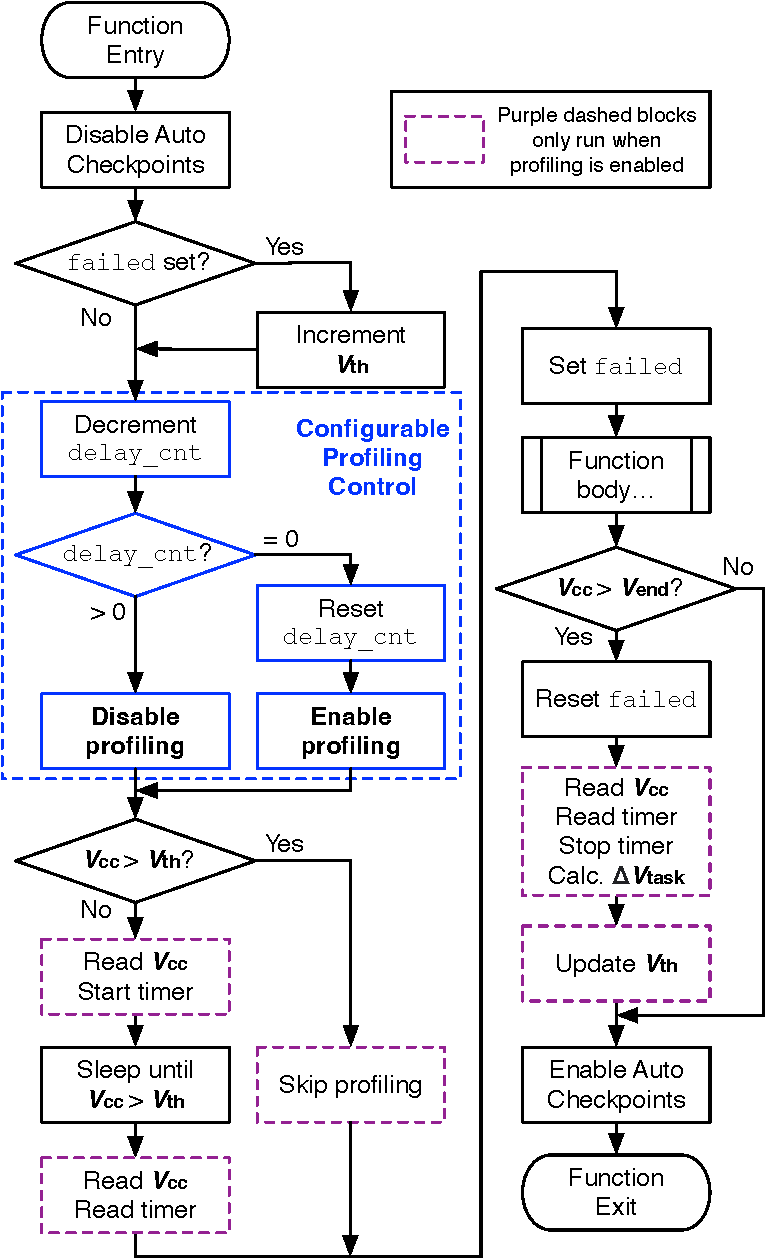
\includegraphics[width=0.8\columnwidth]{ch5_optic/figures/flowchart.pdf}
    \caption{Flowchart of \nn{}'s runtime energy adaptation scheme. The blue blocks represent a configurable control logic to decide when to perform energy profiling. The dashed purple blocks are only run when the profiling is enabled, and represent the profiling operations except for the last one where \nm{V}{th} is updated with the new $\Delta \nmm{V}{task}$. }
    \label{fig:opta_flowchart}
\end{figure}


% optional linear adaptation
% optional multiple configurations (can be similar to multiple atom_func_state)
\subsection{Linear Adaptation}

\subsection{Discussion}

The ability to fall back differentiates it from a "simply-incrementing-threshold" DEBS.
